\documentclass[a4paper,10pt,twocolumn]{article}

\usepackage[header=false,
			handles=false,
			copydocumentclass=false,
			active,
			generate=n-1_rawtext.tex,
			extract-env={document}]{extract}

%====================================PREAMBLE IMPORT====================================

%====================================ENCODING PACKAGES====================================
\usepackage[utf8]{inputenc}%
\usepackage[T1]{fontenc}%
\usepackage{textcomp}%
%====================================ENCODING PACKAGES====================================


%====================================FONT PACKAGES====================================
\usepackage{opensans}%
\usepackage{lmodern}%
%====================================FONT PACKAGES====================================


%====================================UTILITY PACKAGES====================================
\usepackage[english]{babel}%			--> english hyphenation, translation, etc for TeX stuff
\usepackage{csquotes}
\usepackage{import}
\usepackage{pdfpages}%				 	--> inserting .pdf files
\usepackage{amsmath}%				}
\usepackage{amssymb}%				}	--> math
\usepackage{geometry}%
\usepackage{graphicx}%
\usepackage{color}%
\usepackage{float}%
\usepackage{multicol}%					--> handling onecolumn figures
\usepackage{multirow}%				}
\usepackage{booktabs}%				}	--> nice tables
\usepackage{fancyhdr}%				 	--> nice headers
\usepackage{subfig}%					--> creation of subfloats for arrays of images
\usepackage[colorlinks=true,linkcolor=blue,citecolor=kekcolor]{hyperref}%
%====================================UTILITY PACKAGES====================================

%====================================PACKAGE RELATED CONFIGS====================================
\definecolor{kekcolor}{RGB}{15,163,59}
\definecolor{grun}{RGB}{0,127,0}
%\geometry{top=0.75 in, bottom=1in, left=0.75in, right=0.75in,columnsep=0.2in}%
\geometry{top=19mm, bottom=30mm, left=13mm, right=13mm,columnsep=4mm}%
%SOURCE ----> https://www.yumpu.com/en/document/read/48657545/preparation-of-papers-in-two-column-format-for-the-date
\setlength{\headheight}{14pt}%			--> fancyhdr requires a sufficent \headheight
\renewcommand{\arraystretch}{1.1}%		--> correcting for the look of tables (more room between each row)
%====================================PACKAGE RELATED CONFIGS====================================


%====================================GENERAL CONFIGS====================================
\setlength{\parindent}{0pt}%			--> no initial indents
\numberwithin{equation}{section}%		--> the equation counter loops in each succession of section counter
\makeatletter%						}
\@newctr{footnote}[section]%			} 	--> the footnote counter loops in each succession of the page counter
\makeatother%						}
%====================================GENERAL CONFIGS====================================


%====================================OBAMINA FAMILY OPERATORS====================================
\usepackage{obaminaandmore}%
%TexStudio may mark the used package as unkown. Ignore. It's in the folder as obamina_andmore.sty
%====================================OBAMINA FAMILY OPERATORS====================================


%=====================================STYLING THE SECTION TITLES====================================
\usepackage{titlesec}
\titleformat{\section}
{\fsi{12pt}\fsa{sc}\sefo}
{\fsi{13pt}\sefo\textbf{\thesection.}}
{2ex}
{\filcenter}


\titleformat{\subsection}
{\fsi{10pt}\fsa{sc}\sefo}
{\fsi{11pt}\sefo\textbf\thesubsection.}
{2ex}
{\filcenter  }
%====================================STYLING THE SECTION TITLES====================================


%====================================STYLING THE TABLE OF CONTENTS====================================
\usepackage{titletoc}
%\dottedcontents{section}[0pt]{}{2ex}{5cm}
\contentsmargin{1cm}
\titlecontents{section}[0pt]%format and left
			  {\addvspace{16pt}}% above-code
			  {\fse{b}\fsi{15pt}\os\sefo\thecontentslabel \hspace{2ex} }%numbered-entry-format
			  {\fse{b}\fsi{15pt}\os\sefo\thecontentslabel \hspace{2ex} }%numberless-entry-format
			  {\hfill {\fsi{14pt}\sefo \thecontentspage}}%filler-page-format
			  [\addvspace{4pt}]%below-code
			  
%\dottedcontents{subsection}[14ex]%format and left
%			   {\Large}%above-code alias global formatting of the entry
%			   {5ex}%label-width
%			   {5pt}%leader-with
			   
\titlecontents{subsection}[1cm]{}{\Large\thecontentslabel\hspace{3ex}}{\Large}{\hfill {\fsi{14pt}\sefo\thecontentspage}}
			  
%====================================STYLING THE TABLE OF CONTENTS====================================


%====================================FANCYHDR and HEADERS INIT====================================
\pagestyle{fancy}
\fancyhf{}
\renewcommand{\sectionmark}[1]{\markright{#1}}
\renewcommand{\subsectionmark}[1]{}
\fancyhead[LO]{\textbf {\fsi{11pt}\sefo \thesection}.\hspace{2ex}{\scshape \rightmark}}
\fancyhead[RO]{\textbf \thepage}
%====================================FANCYHDR and HEADERS INIT====================================


%====================================FONT COMMANDS====================================
\newcommand{\fsi}[1]{\fontsize{#1}{8pt}}
\newcommand{\fse}[1]{\fontseries{#1}}
\newcommand{\fsa}[1]{\fontshape{#1}}
\newcommand{\sefo}{\selectfont}
\newcommand{\os}{\fontfamily{opensans-TLF}}
\newcommand{\FT}{{\os\sefo FT}}
\newcommand{\IFT}{{\os\sefo IFT}}
%====================================FONT COMMANDS====================================


%====================================NEW COMMANDS====================================
\newcommand{\mypar}{\\[0.4\baselineskip]}
\newcommand{\BHJ}{{\os\sefo BHJ}}
\newcommand{\OSC}{{\os\sefo OSC}}
\newcommand{\BHSC}{{\os\sefo BHSC}}
%====================================NEW COMMANDS====================================


%====================================BIBLIOGRAPHY====================================
\usepackage[backend=biber,style=alphabetic,maxbibnames=10,maxcitenames=3]{biblatex}
%====================================BIBLIOGRAPHY====================================
%====================================PREAMBLE IMPORT====================================


%========================WE NEED LOCAL DEFINITION OF PATH TO BIB========================
\addbibresource{../../0_Bibliography/FPR.bib}
%========================WE NEED LOCAL DEFINITION OF PATH TO BIB========================


\begin{document}\begin{extract*}

\section{Improvements}\label{sec:improvements}
If we look at table~\ref{tab:assemb-table} and assume that $\mathbb{S}_1$ and $\mathbb{S}_2$ could have held two additional cells, then a total of 22 working \BHSC’s could have been assembled. Out of these 22 cells only 5 demonstrated basic functionality. If we want to think about how we can improve our solar cells then we have to discuss how the assembly process can be improved.

\subsection{Tools for the assembly}
When performing any manipulation on a set, we used a pair of tweezers to fixate it. We are certain that the tweezers are a great tool for this type of application, but when it comes to \emph{moving} a set of cells from one table to the other, this can quickly lead to contamination. Performing the spin coating for each active layer, involved grabbing the sets by hand or with the tweezers and moving them. But in order to lift a set with the tweezers at our disposal, the glass substrate had to be held under tension which makes the whole system very sensitive to perturbations. Combined with the fact that this way of holding a set is subject to skill and we were two experimenters, set $\mathbb{S}_4$ dropped in the process of moving it to the spin coater.\mypar
The minimal solution to this problem would the introduction of a bigger pair of tweezers that do not have be spread apart in order to grab a set. But because the tweezers proved to be sufficient for fixating the substrates, we want to propose an established multipurpose tool for moving a set of \BHSC's that is often found in microscopy tool sets.

\begin{figure}[h]\centering
	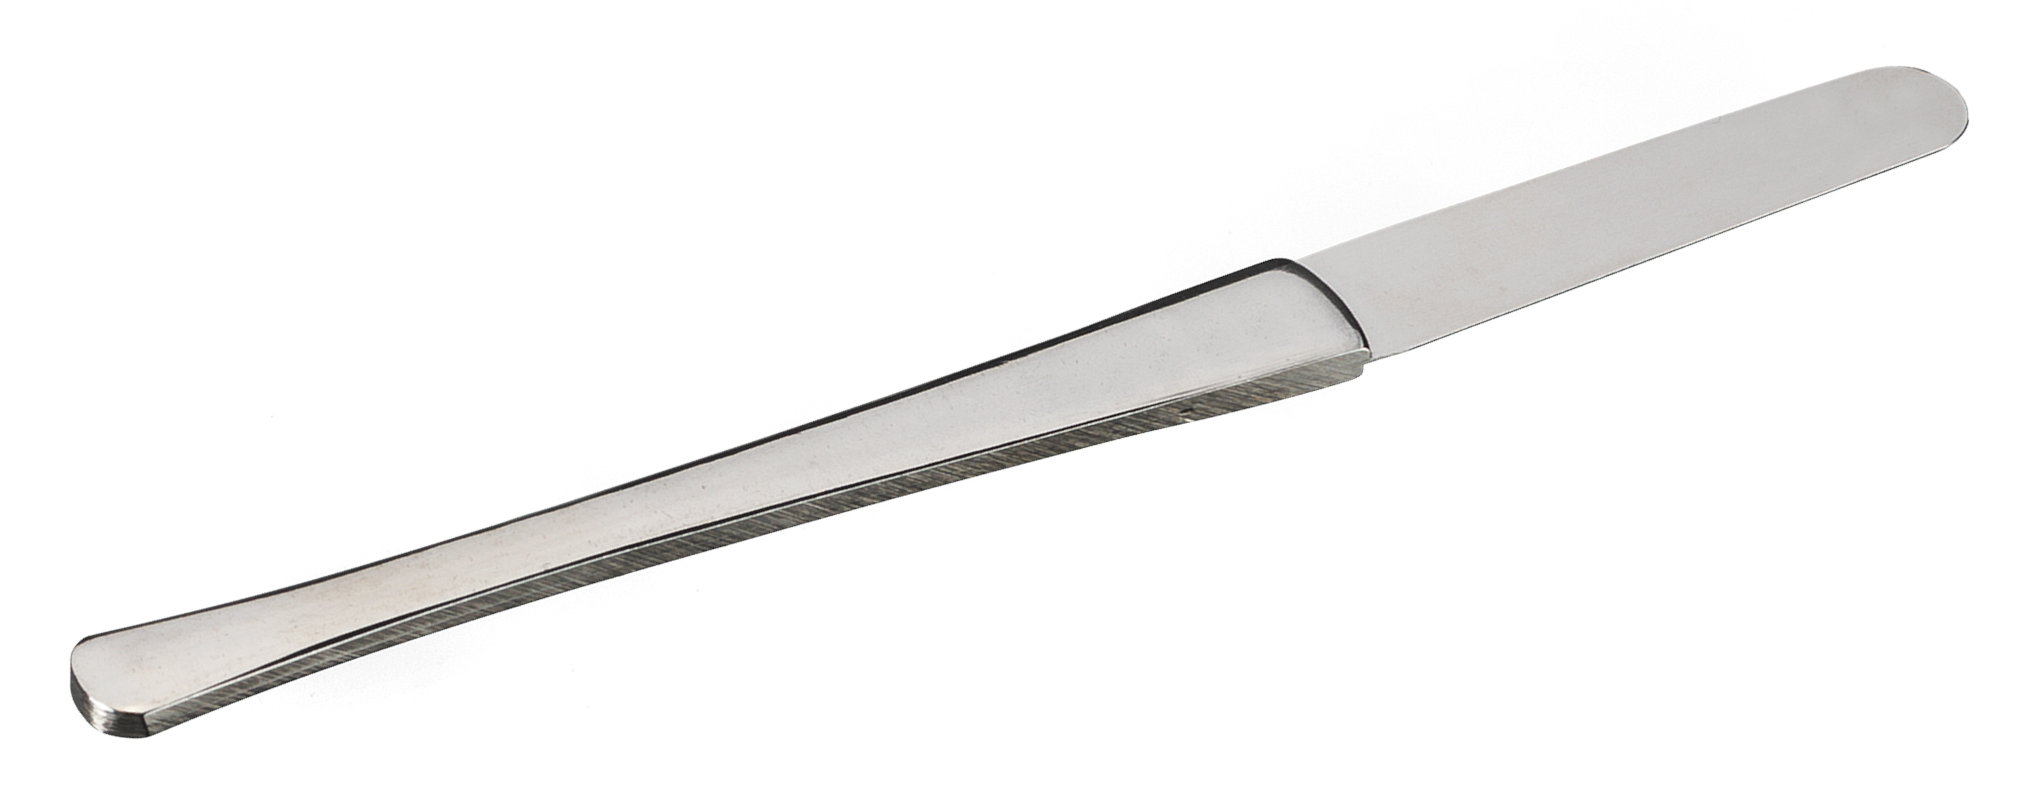
\includegraphics[width=\columnwidth]{../n-1_Pictures/Schnittfaenger.png}
	\caption{Version of a "Schnittfänger" sold in a microscopy tool set made by BRESSER.}
	\label{fig:cutcatcher}
\end{figure}
Figure~\ref{fig:cutcatcher} shows a version of the tool we are talking about. A Schnittfänger\footnote{We did not find a proper translation for it.} is a multipurpose spatula with a flexible and thin blade that is produced in various widths. In our use case and in combination with tweezers, it makes a great tool for picking up the delicate glass substrates or getting it out of the spin coater and holding it without any tension involved.\mypar
As visible in figures~\ref{fig:realblob} and \ref{fig:realblob2}, we also applied silver contacts onto the substrates to establish a better contact when modulating the voltage. This was done by using a brush that was soaked in a silver solution. As the characteristic dimensions of the brush were around three times as big as the width $w$ of the ITO stripe, we had poor overall control when applying the silver contacts. This resulted in the situation depicted in figure~\ref{fig:realblob3} where a drop of silver came off the brush and dried on the substrates surface.

\begin{figure}[h]\centering
	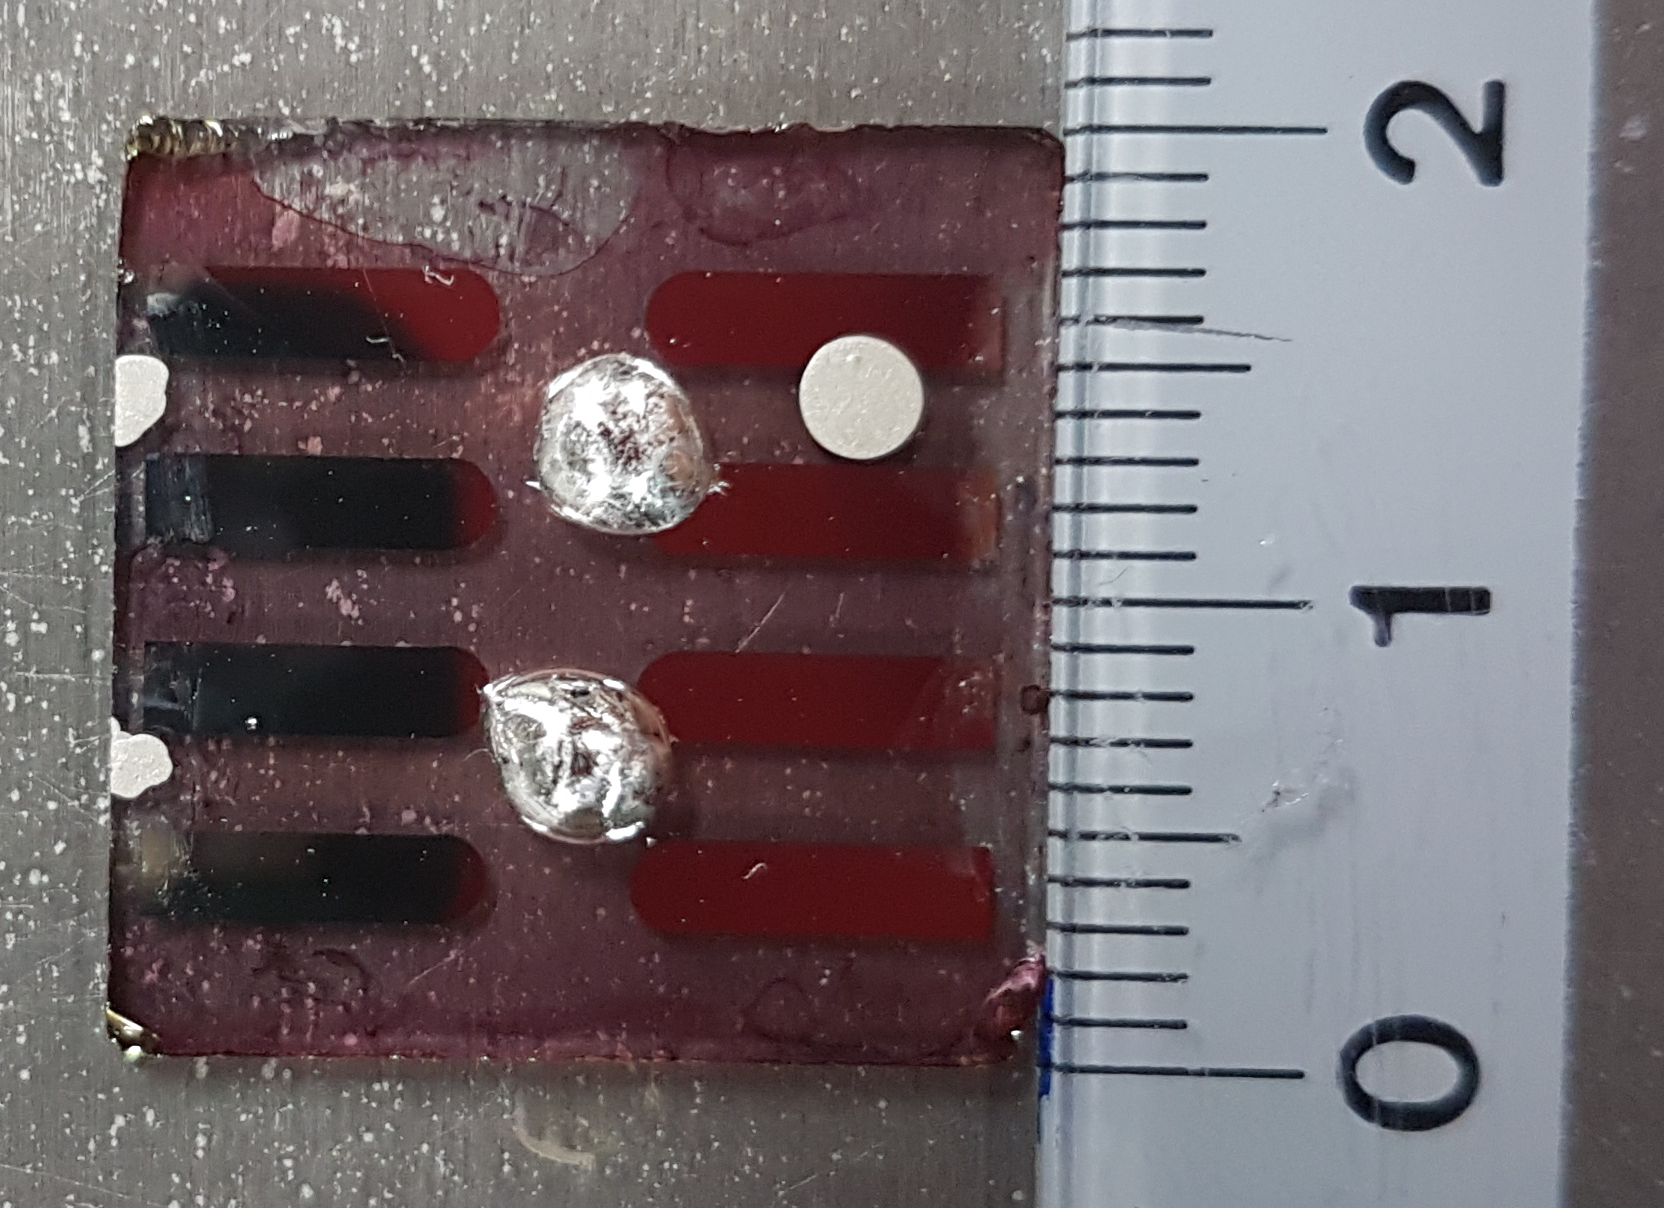
\includegraphics[width=0.9\columnwidth]{../n-1_Pictures/cell1.png}
	\caption{Assembled set $\mathbb{S}_1$ with ruler next to it. A drop of silver contact is visible in the upper right corner of the prepared substrate.}
	\label{fig:realblob3}
\end{figure}

As the silver solution in the brush also dried out very fast, applying homogeneous contacts proved to be very difficult. An example is visible in figure~\ref{fig:realblob2} in the upper right corner of the substrate where we did not manage to recover a homogeneous contact.\mypar
We propose the use of disposable pipettes\footnote{Disposable pipette tips would be a great alternative.} in combination with a brush which contains a minimal amount of silver solution on it. Disposable pipettes are a standard in every chemistry lab and with the ability to control the amount of silver brought onto the substrate one can spread this amount evenly with the brush to achieve homogeneous and precise contacts of appropriate thickness.

\subsection{Pressure in evaporation process}

With $p_0$ described in section~\ref{subsec:therm-eval} we met the requirements of a base pressure of $p_0<10^{-7}\;\text{mbar}$ (see \cite{labdesc} section 3.2). But we positioned the sample holder over the filament when the pressure was unstable and continued to increase the current flowing through the aluminum filament. This resulted in pressures of around $1.6(1)\cdot10^{-6}\;\text{mbar}$.\mypar
Given the drawbacks of insufficient pressures mentioned in \cite{labdesc}, waiting longer for the pressure to stabilize and decrease might prove to have a significant impact on performance and functionality.

\subsection{External information at hand}\label{subsec:broedelsec}

The calibration of the SUN~2000 was carried out firstly by the Laser~Point PD-500-D9-VIS photo diode. Referring to it's manual \cite{reracat}, which we could not find at the time of the lab, the photo diodes aperture diameter is
\begin{equation*}
	d^\prime_p = 9.5(1)\;\text{mm}\quad\text{with which}\quad A^\prime_p = 70.9(15)\;\text{mm}^2.
\end{equation*}

Using this as the illuminated area of the photo diode would result in an irradiance of
\begin{equation*}
	S^\prime_{p0} = 1.157(28)\;\frac{\text{mW}}{\text{mm}^2}.
\end{equation*}
As this irradience is around 16\% higher than the result, for which we would have declared the SUN~2000 to be calibrated, we would have changed the adjustable current on the SUN~2000. In the end we tested the calibration with the Rera~RQN3686 silicon cell with which we declared the solar simulator to be calibrated. We propose to perform more detailed testing of the Laser~Point diode as it is not clear how the calibration should have been carried out without the silicon reference cell.


\end{extract*}
\end{document}